\begin{referat}{Wstęp do teorii grafów, twierdzenie Ramseya}{Grzegorz Świrski}

\begin{teoria}
\subsubsection{Podstawowe pojęcia i definicje}

\textbf{Grafem} nazywamy zbiór \textbf{wierzchołków} i połączeń między nimi - \textbf{krawędzi}. Wierzchołki grafów zazwyczaj są numerowane i stanowią reprezentację jakiś obiektów. Krawędzie przedstawiają relacje między tymi obiektami. Grafy możemy podzielić na \textbf{nieskierowane} i \textbf{skierowane}.

\textbf{Graf nieskierowany} to uporządkowana para $\mathbf{G}=\left( V,E \right)$, gdzie:
\begin{itemize}
 \item $\mathbf{V}$ jest zbiorem wierzchołków
 \item $\mathbf{E}$ jest rodziną (zbiorem zbiorów) krawędzi: 
    $$E\subseteq \{ \{u,v\} : u,v \in V\}$$
\end{itemize}

Wśród grafów nieskierowanych wyróżniamy \textbf{grafy proste}, w których nie występują pętle (krawędzie wychodzące i wchodzące do tego samego wierzchołka) oraz wielokrotne krawędzie między tymi samymi wierzchołkami.

\textbf{Grafy skierowane} różnią się tym, że każda krawędź ma swój zwrot. Istnienie połączenia z wierzchołka 1 do wierzchołka 2 wcale nie implikuje połączenia z wierzchołka 2 do wierzchołka 1.

Formalnie graf skierowany definiujemy jako uporządkowaną parę $\mathbf{G}=\left( V,A \right)$, gdzie:
\begin{itemize}
 \item $\mathbf{V}$ jest zbiorem wierzchołków
 \item $\mathbf{A}$ jest zbiorem uporządkowanych par różnych wierzchołków ze zbioru V, zwanych \textbf{krawędziami skierowanymi}: $A\subseteq V \times V$.
 Przyjmuje się, że krawędź $e = \left( x, y \right)$ jest skierowana z wierzchołka x do wierzchołka y. Innymi słowy wychodzi z wierzchołka x, a wchodzi do y.
\end{itemize}

Czasem wprowadza się pojęcie \textbf{grafu mieszanego} zawierającego zarówno krawędzie skierowane jak i nieskierowane.

Najprostszą w odbiorze (dla człowieka) jest reprezentacja na płaszczyźnie.
\begin{figure}[h]
  \centering
  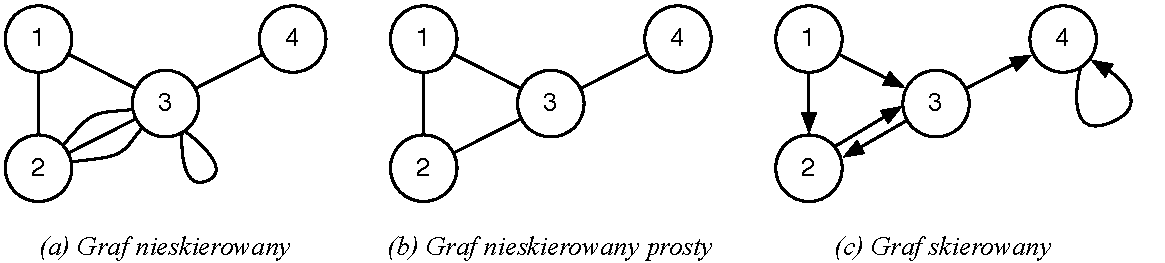
\includegraphics[scale=0.65]{./swirski/graph_types.pdf}
  \caption{Reprezentacja grafu na płaszczyźnie}
\end{figure}

\textbf{Stopień wierzchołka} $v$ w grafie $\mathbf{G}$ to liczba krawędzi incydentnych (mających swój początek lub koniec w tym wierzchołku) z v. Oznaczamy go jako ${\sf deg} \ v$ lub $d(v)$.

\textbf{Podgraf} grafu $\mathbf{G}$ to graf $\mathbf{H}$, w którym ${\sf V}\!\left(\mathbf{H}\right)\subseteq{\sf V}\!\left(\mathbf{G}\right)$ i ${\sf E}\!\left(\mathbf{H}\right)\subseteq{\sf E}\!\left(\mathbf{G}\right)$, gdzie $V(X)$ to zbiór wierzchołków grafu $X$, $E(X)$ to zbiór krawędzi grafu $X$.

\textbf{Restrykcja} grafu $\mathbf{G}$ do podzbioru $X\subseteq V$ to $\mathbf{G}|_X=\left( X,\left\lbrace vw:v,w\in X \right\rbrace \right)$.

\textbf{Podgraf indukowany} grafu $\mathbf{G}$ to graf będący restrykcją grafu $\mathbf{G}$,

\textbf{Graf pusty} to graf bez krawędzi zwany także \emph{antykliką} lub \emph{grafem niezależnym}. Antyklikę o $n$ wierzchołkach będziemy oznaczać przez $\mathcal{A}_{n}$

\textbf{Graf pełny} (inaczej: \emph{klika}) to graf, w którym każde dwa wierzchołki połączone są krawędzią. Klikę o $n$ wierzchołkach będziemy oznaczać przez $\mathcal{K}_{n}$


\begin{twierdzenie}{Liczba krawędzi w klice}
Liczba krawędzi w klice $\mathcal{K}_{n}$ wynosi $\frac{n(n-1)}{2}$
\end{twierdzenie}

\begin{dowod}
Dowód przeprowadzimy indukcyjnie:
\begin{enumerate}
 \item Zauważamy, że dla liczby wierzchołków równej 0 lub 1 liczba krawędzi wynosi 0.
 \item Założenie: $|E(K_{n})| = \frac{n(n-1)}{2}$\\
 Teza: $|E(K_{n+1})| = \frac{n(n+1)}{2}$\\
 Mając graf pełny o $n$ wierzchołkach dodajmy wierzchołek i uzupełnijmy krawędzie, aby znowu otrzymać graf pełny o $n+1$ wierzchołkach. Widzimy, że dostaliśmy $n$ nowych krawędzi.\\
 Korzystając z założenia otrzymujemy:
 $$ \frac{n(n-1)}{2} + n = \frac{n(n+1)}{2} $$
\end{enumerate}
$1, 2 \implies$ liczba krawędzi w klice $\mathcal{K}_{n}$ wynosi $\frac{n(n-1)}{2}$
\end{dowod}

\textbf{Marszruta} w grafie $G$ z wierzchołka $u$ do wierzchołka $w$ to skończony ciąg krawędzi w postaci $(uv_1, v_1,v_2,\ldots,v_{k-1}w)$. W skrócie marszrutę taką oznaczamy przez $u\to v_1\to v_2\to\ldots\to v_{k-1}\to w$. Wierzchołek $u$ nazywać będziemy \emph{początkowym}, a $w$ \emph{końcowym}. Jeżeli marszrutę zdefiniowano na krawędziach skierowanych (uwzględniając kierunek w jakim możemy się poruszać !), to mówimy o \emph{marszrucie skierowanej}.

\textbf{Długość marszruty} $u\to v_1\to v_2\to\ldots\to v_{k-1}\to w$
to liczba jej krawędzi.

\textbf{Marszruta zamknięta} to marszruta kończąca się w punkcie wyjścia, 
czyli taka, w której $u=w$

\textbf{Droga} to marszruta bez powtarzających się wierzchołków. Droga nazywana jest też często \textbf{ścieżką}.

\textbf{Cykl} to marszruta zamknięta, w której jedynym powtarzającym się wierzchołkiem jest jej początek (będący oczywiście również jej końcem).

\textbf{Graf spójny} to graf, w którym między dwoma dowolnymi wierzchołkami istnieje droga. \textbf{Graf niespójny} to graf, który nie jest spójny.

\textbf{Spójna składowa} grafu $\mathbf{G}=\left(V,E\right)$
to maksymalny (w sensie ilości wierzchołków) podzbiór $X\subseteq V$,
indukujący graf spójny $\mathbf{G}|_X$

\textbf{Wierzchołek izolowany} to wierzchołek nie posiadający sąsiadów.

\textbf{Klasyczne kolorowanie grafu} (inaczej wierzchołkowe kolorowanie grafu) polega na przypisaniu każdemu wierzchołkowi pewnej liczby naturalnej. Ze względów historycznych oraz dla lepszego zobrazowania problemu mówi się o kolorowaniu, przy czym różnym kolorom odpowiadają różne liczby. \textbf{Legalnym pokolorowaniem grafu} nazywamy takie kolorowanie, gdzie końcom żadnej krawędzi nie przyporządkowano tego samego koloru.

\textbf{Kolorowanie krawędzi} polega na przyporządkowaniu krawędziom (zamiast wierzchołków) liczb naturalnych oznaczających kolory. \textbf{Kolorowaniem legalnym} (właściwym, prawidłowym) nazywamy kolorowanie w którym żaden wierzchołek nie ma kilku krawędzi tego samego koloru.

\textbf{Optymalnym kolorowaniem grafu} nazywamy legalne pokolorowanie tego grafu przy użyciu najmniejszej możliwej liczby kolorów. \textbf{Liczbą chromatyczną} grafu $G$ nazywamy liczbę $\chi(G)$ będącą ilością kolorów w optymalnym kolorowaniu.

\subsubsection{Cykl Eulera}
Nazwa pochodzi od nazwiska matematyka Leonharda Eulera, który jako jeden z pierwszych zajmował się problematyką dróg w grafach. 

\textbf{Ścieżka Eulera} to marszruta (niekoniecznie zamknięta) przechodząca przez każdą krawędź grafu dokładnie raz.

\textbf{Cykl Eulera} to \textbf{zamknięta} marszruta przechodząca przez każdą krawędź grafu dokładnie raz.

\textbf{Graf półeulerowski} to graf posiadający ścieżkę Eulera.

\textbf{Graf eulerowski} to graf posiadający cykl Eulera.

\begin{figure}[h]
  \centering
  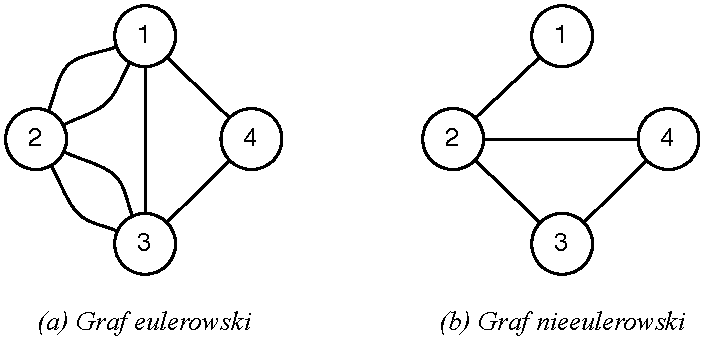
\includegraphics[scale=0.65]{./swirski/eulerian_graphs.pdf}
\end{figure}

Graf na rysunku (a) posiada cykl Eulera $4\to 1\to 2\to 3 \to 1 \to 2\to 3\to 4$, zaś graf (b) nie jest eulerowski, bo jeżeli wejdzie się do wierzchołka $1$, to już nie będzie można z niego wyjść; jeśli zaś rozpoczęlibyśmy naszą marszrutę z wierzchołka $1$ to nie będzie można doń powrócić.

\begin{twierdzenie}{Graf eulerowski}
Graf nieskierowany $G = (V, E)$ jest eulerowski wtedy i tylko wtedy, gdy jest spójny i stopień każdego wierzchołka jest parzysty.
\end{twierdzenie}

\begin{twierdzenie}{Graf półeulerowski}
Jeżeli graf nieskierowany $G = (V, E)$ jest spójny i najwyżej dwa wierzchołki mają stopień nieparzysty to jest możliwe zbudowanie ścieżki Eulera, która nie jest zamknięta - graf jest półeulerowski (pseudoeulerowski).
\end{twierdzenie}

\begin{twierdzenie}{Droga Eulera}
Graf skierowany posiada drogę Eulera, gdy wszystkie wierzchołki z wyjątkiem dwóch mają takie same stopnie wychodzące i wchodzące, w jednym z tych dwóch wierzchołków stopień wychodzący jest o 1 większy niż wchodzący a w drugim odwrotnie.
\end{twierdzenie}

\subsubsection{Cykl Hamiltona}
\textbf{Ścieżka Hamiltona} to ścieżka przechodząca przez wszystkie wierzchołki, każdy odwiedzając tylko jeden raz.

\textbf{Cykl Hamiltona} to cykl przechodzący przez wszystkie wierzchołki grafu (czyli marszruta zamknięta odwiedzająca każdy wierzchołek dokładnie raz).

\textbf{Graf hamiltonowski} to graf posiadający cykl Hamiltona.

W odróżnieniu od grafów eulerowskich, grafy hamiltonowskie nie posiadają prostej i szybkiej w użyciu charakteryzacji. Są natomiast znane pewne warunki wystarczające na to, by graf był hamiltonowski. Jednym z ciekawszych takich warunków wystarczających jest warunek wykorzystujący jedynie stopnie wierzchołków. Przedstawiony jest w postaci następującego twierdzenia.

\begin{twierdzenie}{Graf hamiltonowski}
Jeśli w grafie prostym $\mathbf{G}=\left( V,E \right)$ o co najmniej $3$ wierzchołkach dowolne dwa niesąsiednie wierzchołki $u$ i $w$ spełniają $\deg{v}+\deg{w}\geq \left\vert V \right\vert$, to graf $G$ jest hamiltonowski.
\end{twierdzenie}

\subsubsection{Twierdzenie Ramseya}
Głównym zagadnieniem tego podrozdziału będzie pytanie typu: jak bardzo liczny musi być zbiór, by wystąpiła w nim pożądana konfiguracja. Zacznijmy od twierdzenia będącego dość oczywistym.

Mając $m$ przedmiotów, które chcemy umieścić w $n$ szufladach, przy czym $m > n$, to w co najmniej jednej szufladzie znajdzie się więcej niż jeden przedmiot.

\begin{twierdzenie}{Zasada szufladkowa}
Jeżeli zbiór $X$ liczy sobie $m$ elementów i $X = X_{1} \cup X_{2} \cup... \cup X_{n}$ i $m > n$, to któryś ze zbiorów $X_{i}$ musi zawierać przynajmniej dwa elementy.
\end{twierdzenie}

W oparciu o powyższą zasadę łatwo pokazać, że co najmniej dwóch mieszkańców Warszawy ma tę samą liczbę włosów na głowie. Rzeczywiście, typowa głowa posiada 150 000 włosów, rozsądnie więc będzie przyjąć liczbę 500 000 jako górną granicę. Warszawa liczy sobie ponad 1 000 000 mieszkańców. Weźmy 500 000 szufladek ponumerowanych liczbami naturalnymi od 1 do 500 000 i wkładajmy do szufladki o danym numerze osoby, które mają taką samą liczbę włosów na głowie jak numer szufladki. Ponieważ osób jest ponad 1 000 000, a szufladek 500 000, z naszej zasady wynika, że w jednej szufladce muszą znaleźć się co najmniej dwie osoby.

Bardziej dociekliwi zauważyli zapewne, że osób mamy \textbf{ponad} 1 000 000, dlatego taką samą ilość włosów będą miały co najmniej 3 osoby.

\begin{twierdzenie}{Uogólniona zasada szufladkowa}
Dla dowolnej liczby $q \in \mathbf{N}$, jeśli $X = X_{1} \cup X_{2} \cup... \cup X_{n}$ oraz $|X| \geq (q-1)n + 1$, to dla któregoś $i$ mamy $X_{i} \geq q$.
\end{twierdzenie}

\begin{dowod}
Wykorzystując założenia twierdzenia otrzymujemy następujące oszacowanie:

$$(q-1)n+1\leq\left\vert X \right\vert =\left\vert X_1\cup\ldots\cup X_n \right\vert \leq\left\vert X_1 \right\vert+\ldots+\left\vert X_n \right\vert \leq n\cdot \max_{i=1,\ldots, n}{\left\vert X_i \right\vert}.$$

Tak więc
$$(q-1)+\frac{1}{n}=\frac{(q-1)n+1}{n}\leq\max_{i=1,\ldots, n}{\left\vert X_i \right\vert}$$

Ponieważ moce zbiorów $X_{i}$ są liczbami całkowitymi otrzymujemy, że ta maksymalna musi wynosić co najmniej $q$.
\end{dowod}

Pokażmy, że jeżeli w klasie jest 40 uczniów to co najmniej 4 z nich obchodzi urodziny w tym samym miesiącu. Oczywistym jest, że zastosujemy tutaj zasadę szufladkową Dirichleta.

Do wzoru $|X| \geq (q-1)n + 1$ podstawiamy $q = 4$ (poszukiwana zawartość szuflady) i $n = 12$ (liczba miesięcy jest liczbą szufladek) otrzymując $|X| \geq 37$. $|X| = 40$ jak najbardziej spełnia powyższą nierówność.


Weźmy graf $K_{6}$ z dwukolorowymi krawędziami. Jakkolwiek byśmy tych krawędzi nie pokolorowali, \emph{musi} się z w nim znaleźć monochromatyczny (jednego koloru) trójkąt. Nie dotyczy to natomiast grafu $K_{5}$.
\begin{figure}[h]
 \centering
 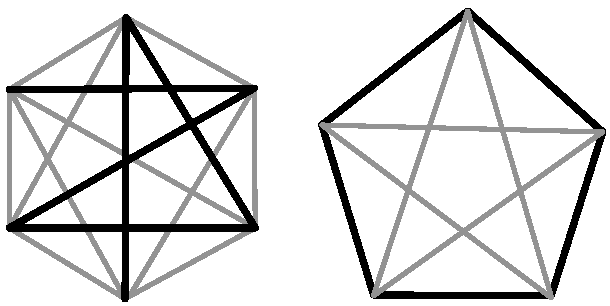
\includegraphics[scale=0.6]{./swirski/ramsey_example.pdf}
\end{figure}

\begin{twierdzenie}{Liczba Ramseya}
Dla liczb naturalnych $k,l \geq 2$ istnieje najmniejsza liczba $R\left(k,l\right)$ (znana jako liczba Ramseya) taka, że dwu-kolorowego grafu pełny $K_{R\left(k,l\right)}$ będzie zawierał monochromatyczny podgraf $K_{k}$ lub $K_{l}$.\\
Lub nieco inaczej: dla dowolnych liczb naturalnych $k$ i $l$ istnieje liczba naturalna $R\left(k,l\right)$ taka, że graf z $R\left(k, l\right)$ wierzchołkami będzie zawierał klikę z co najmniej $k$ wierzchołkami lub antyklikę o co najmniej $l$ wierzchołkach.
\end{twierdzenie}

\begin{dowod}
Dowód poprowadzimy przez indukcję po $k+l$.

Dla $k, l \leq 2$ sprawa jest trywialna:
\begin{align*}
R\left(1, x\right) &= R\left(x, 1\right) = 1\\
R\left(2, x\right) &= R\left(x, 2\right) = x
\end{align*}

To rozpocznie naszą indukcję. Aby dowieść, że $R(r,s)$ istnieje znajdziemy przedział, w jakiej musi znaleźć się jej wartość. \\
Założenie: istnieje $R(r-1, s)$ i $R(r, s-1)$ \\
Teza: $R(r, s) \leq R(r-1,s) + R(r,s-1)$

Rozważmy graf pełny $K_{R(r-1,s) + R(r, s-1)}$. Wybieramy dowolny jego wierzchołek $v$. Dzielimy resztę wierzchołków na zbiory $M$ i $N$ w zależności od koloru krawędzi z $v$.

Ponieważ graf ma $R(r-1,s) + R(r, s-1) = |M| + |N| + 1$ wierzchołków, to albo $|M| \geq R(r-1,s)$ albo $|N| \geq R(r, s-1)$. W pierwszym przypadku, jeżeli $M$ zawiera czerwony graf pełny $K_s$ to zawiera go również oryginalny graf i skończyliśmy dowód. W przeciwnym wypadku $M$ zawiera niebieską klikę $K_{r-1}$ oraz $M \cup{} \{v\}$ zawiera niebieską klikę $K_r$ z definicji $M$, co kończy dowód kroku indukcyjnego. Dla $N$ postępujemy analogicznie.

Z zasady indukcji otrzymujemy, że twierdzenie jest prawdziwe.
\end{dowod}

Istnieje również uogólnienie dla dowolnej, skończonej liczby kolorów i liczbie wierzchołków równej $R\left(n_{1},..., n_{c}\right)$

\textit{Przykłady liczb Ramseya}

\begin{align*}
&R(3,3) = 6\\
&R(3,4) = 9\\
&R(3,5) = 14\\
&R(4,4) = 18\\
&R(3,6) = 18\\
&R(3,7) = 23\\
&R(3,8) = 28\\
&R(3,9) = 36\\
&R(4,5) = 25\\
43 \leq &R(5,5)\leq 49\\
109 \leq &R(6,6)\leq 165\\
205 \leq &R(7,7)\leq 540\\
282 \leq &R(8,8)\leq 1870\\
565 \leq &R(9,9)\leq 6588\\
798 \leq &R(10,10)\leq 23581
\end{align*}
Jak widać ustalenie dokładnej liczby (nawet przy małych argumentach) jest bardzo trudne. Przewiduje się nawet, że dokładne rozwiązanie dla $R(6,6)$ nie będzie nigdy znane.

Na pewno jednak, mając graf o liczbie wierzchołków większej lub równej górnemu kryterium, twierdzenie zostanie spełnione.

\begin{twierdzenie}{Rozszerzone twierdzenie Ramseya}
Weźmy naturalne $m, n \geq 2$. Wśród dowolnych $2^{m+n}$ ludzi istnieje albo $m$ ludzi, którzy się parami znają, albo $n$ ludzi, którzy się parami nie znają.
\end{twierdzenie}

\begin{dowod}
Jako $P(m, n)$ oznaczmy zdanie,,Pośród dowolnych $2^{m+n}$ wierzchołków istnieje albo graf pełny $K_m$, albo antyklika $A_n$''.

Dodatkowo, niech $Q(s)$ oznacza,,$P(m,n)$ jest prawdziwe dla dowolnych naturalnych $m,n \geq 2$ i $m+n = s$''. Poprowadzimy indukcję po $s \geq 4$.

Przypadek początkowy: $s = 4$, $m=n=2$. Z twierdzenia Ramseya wiemy, że pośród $2^{2+2} = 16$ znajdziemy pasujące dwa wierzchołki. Dowiedliśmy, że $Q(4)$ jest prawdziwe.

Założenie: $s > 4, Q(4), Q(5), \ldots, Q(s-1)$ są prawdziwe

Teza: $Q(s)$ jest prawdziwe

\emph{Przypadek 1:} $m=2, n=s-2$ Weźmy $n$ wierzchołków (wiemy, że $2^n > n$). Albo nie istnieje wśród nich żadne połączenie, albo istnieje co najmniej jedno. W obu wypadkach udowodniliśmy $P(m,n)$.

\emph{Przypadek 2:} $n=2, m = s-2$ Analogicznie jak przypadek 1.

\emph{Przypadek 3:} $m,n > 2$. Załóżmy, że wierzchołek $v_1$ ma $x$ krawędzi; pozostałe $y = 2^{m+n} - 1 - n$ nie mają z nim połączenia. Oczywistym jest, że albo $x \geq 2^{m+n-1}$ albo $y \geq 2^{m+n-1}$.

Rozważmy pierwszy przypadek ze zbiorem $S$ jako zbiorem wierzchołków sąsiadujących wierzchołka $v_1$. Z założenia indukcyjnego dla $m-1, n$ mamy albo $m-1$ wierzchołków w zbiorze $S$, które są połączone z $v_1$ (czyli razem z $v_1$ otrzymujemy klikę $K_n$), lub $m$ wierzchołków w $S$, które tworzą graf pusty $A_n$. W obu wypadkach udowodniliśmy $P(m,n)$. Przypadek $y \geq 2^{m+n-1}$ rozwiązujemy analogicznie, co kończy dowód kroku indukcyjnego.

Udowodniliśmy, że twierdzenie jest prawdziwe.
\end{dowod}

\end{teoria}

\subsection{Zadania}

\subsubsection{Zadanie 1}
\textbf{Niech $G$ będzie grafem prostym z co najmniej dwoma wierzchołkami. Wykaż, że  $G$ zawiera dwa wierzchołki tego samego stopnia.}
\zrodlo{http://osilek.mimuw.edu.pl}

Niech $\mathbf{G}$ ma $n\geq 2$ wierzchołków. 
Wierzchołek $v\in{\sf V}\!\left(\mathbf{G}\right)$ 
nie może mieć więcej niż $\left\vert {\sf V}\!\left(\mathbf{G}\right)-\left\lbrace v \right\rbrace \right\vert=n-1$ sąsiadów. 
Stopień dowolnego wierzchołka z ${\sf V}\!\left(\mathbf{G}\right)$ 
leży więc w zbiorze $\left\lbrace 0,1,2,\ldots,n-1 \right\rbrace$. 
Jeśli jakiś wierzchołek ma stopień $0$, czyli jest izolowany, 
to każdy inny wierzchołek może mieć co najwyżej $n-2$ sąsiadów. 
Z kolei gdyby istniał punkt $w$  o stopniu równym $n-1$, 
to każdy wierzchołek ze zbioru ${\sf V}\!\left(\mathbf{G}\right)-\left\lbrace w \right\rbrace$ 
byłby sąsiadem $w$, więc nie mogłby mieć stopnia równego $0$. 
Zbiór $S$ stopni wierzchołków grafu $\mathbf{G}$ zawiera się więc albo w zbiorze 
$\left\lbrace 0,1,2,\ldots,n-2 \right\rbrace$, albo w  $\left\lbrace 1,2,3,\ldots,n-1 \right\rbrace$, 
więc $S$ jest co najwyżej $\left( n-1 \right)$ -elementowy. 
Wszystkich wierzchołków jest $n$, 
więc z Zasady Szufladkowej Dirichleta otrzymujemy, 
że istnieją dwa wierzchołki o tym samym stopniu.
\begin{flushright}
$\square$
\end{flushright}

\subsubsection{Zadanie 2}
\textbf{Niech $n$ będzie dodatnią liczbą całkowitą parzystą. Udowodnić, że istnieje permutacja $ (x_1,x_2, \ldots,x_n) $ zbioru $ \{1,2,\ldots,n\} $, spełniająca dla każdego $ i \in \{1,2,\ldots,n\} $ warunek:
$x_{i+1} $ jest jedną z liczb $ 2x_i $, $ 2x_i-1 $, $ 2x_i-n $, $ 2x_i-n-1$
przy czym $ x_{n+1} = x_1 $.}
\zrodlo{LIV OM}

Przyjmijmy oznaczenia: 
$$f(x)=
\left\{\begin{array}{ll}
2x&\textrm{gdy}\ x \leq n/2,\\
2x-n&\textrm{gdy}\ x>n/2,\\
\end{array}\right.$$
$$ g(x)= f(x)-1 $$

Rozważamy graf skierowany o $ n $ wierzchołkach ponumerowanych jako $ 1,2,\ldots,n $, w którym z punktu (wierzchołka) $ x $ wychodzą dwie zorientowane krawędzie: do punktu $ f(x) $ i do $ g(x) $. Teza sprowadza się do istnienia zamkniętej ścieżki, przechodzącej przez każdy wierzchołek dokładnie jeden raz (cyklu Hamiltona).

Startując od wierzchołka o numerze $ 1 $ i działając funkcjami $ f $, $ g $, możemy uzyskać: w jednym kroku - punkty $ 1 $ i $ 2 $; w dwóch krokach - punkty $ 1 $, $ 2 $, $ 3 $, $ 4 $; w trzech krokach - punkty od $ 1 $ do $ 8 $; itd. Widać, że każdy punkt jest osiągalny z wierzchołka $ 1 $.

Niech $ S: x_1 \to x_2 \to \ldots \to x_m $ będzie najdłuższą ścieżką, przechodzącą przez różne wierzchołki, wśród których jest wierzchołek o numerze $ 1 $. Obie wychodzące z punktu $ x_m $ krawędzie trafiają w pewne punkty ścieżki $ S $ (w przeciwnym razie ścieżkę dałoby się przedłużyć). Mamy więc krawędzie $ x_m \to x_k $, $ x_m \to x_\ell $ ($ k,\ell \leq m $, $ k \neq \ell $); niech np. $ f (x_m) = x_k $, $ g(x_m) = x_\ell $.

Przypuśćmy, że $ k,\ell > 1 $. Wówczas
$$ x_k \in \{f (x_{k-1}),g(x_{k-1})\},\  x_\ell \in \{f (x_{\ell-1}),g(x_{\ell-1})\}. $$

Funkcja $ f $ przyjmuje tylko wartości parzyste, a $ g $ wartości nieparzyste. Ponadto każda z równości $ f (x) = f (y) $ i $ g(x) = g(y) $ implikuje $ x \equiv y (\mathrm{mod}\ n/2) $. Zatem $$ x_k=f(x_{k-1})=f(x_m),\ x_\ell=g(x_{\ell-1})=g(x_m), $$ skąd $ x_m \equiv x_{k-1} \equiv x_{\ell-1} (\mathrm{mod}\ n/2) $ - sprzeczność, bo $ x_m, x_{k-1}, x_{\ell- 1} $ są trzema różnymi liczbami ze zbioru $ \{1, 2, \ldots, n\} $.

Zatem $ k = 1 $ lub $ \ell =1 $, co oznacza, że $ x_m \to x_1 $ jest krawędzią grafu. Uzupełnia ona ścieżkę $ S $ do zamkniętego cyklu. Załóżmy, że poza nią pozostały jakieś wierzchołki grafu. Są one osiągalne z wierzchołka o numerze $ 1 $ (leżącego na ścieżce $ S $). Zatem z pewnego punktu tej ścieżki, $ x_p $, musi wychodzić krawędź do punktu $ y $ leżącego poza nią. Wtedy $ x_{p+1} \to \ldots \to x_m \to x_1 \to \ldots \to x_p \to y $ jest ścieżką przechodzącą przez $ m+1 $ różnych wierzchołków (wśród których jest punkt $ 1 $), wbrew maksymalności $ m $.

\textbf{Wniosek} ścieżka $ S $, uzupełniona krawędzią $ x_m \to x_1 $, jest cyklem przechodzącym przez wszystkie wierzchołki grafu.
\begin{flushright}
$\square$
\end{flushright}

\subsubsection{Zadanie 3}
\textbf{Na okręgu obrano $n>2$ punktów i każdy z nich połączono odcinkiem z każdym innym. Czy można wykreślić wszystkie te odcinki jednym ciągiem, tzn. tak, żeby koniec pierwszego odcinka był początkiem drugiego, koniec drugiego - początkiem trzeciego itd., i żeby przy tym koniec ostatniego odcinka był początkiem pierwszego?}
\zrodlo{XVI OM}

Założenie, że wszystkie punkty leżą na okręgu można zastąpić założeniem słabszym - żadne 3 punkty nie są współliniowe. Widzimy więc, że każdy punkt możemy przedstawić jako wierzchołek, natomiast odcinki między nimi jako krawędzie. Otrzymujemy graf pełny (klikę) $K_n$.

Graf jest jednokreślny (można narysować krawędzie nie odrywając ołówka) wtedy i tylko wtedy, gdy zawiera ścieżkę Eulera (wynika to w sposób oczywisty z definicji).

Widzimy, że z każdego wierzchołka wychodzi $(n-1)$ krawędzi. Stopień każdego wierzchołka jest więc równy $(n-1)$. Dodatkowo, ponieważ $n > 2$, niemożliwa jest sytuacja, gdzie co najwyżej dwa wierzchołki mają nieparzysty stopień, a pozostałe parzysty. Z tego wynika, że $(n - 1)$ musi być liczbą parzystą, czyli $n$ musi być nieparzyste.

Udowodniliśmy, że poszukiwane odcinki możemy wykreślić jednym ciągiem wtedy i tylko wtedy, gdy $n$ jest liczbą nieparzystą.\\


\subsubsection{Zadanie 4}
\textbf{Na płaszczyźnie obrano 6 punktów, z których żadne 3 nie leżą na jednej prostej i wykreślono wszystkie odcinki łączące parami te punkty. Niektóre z odcinków wykreślono przy tym kolorem czerwonym, a inne niebieskim. Dowieść, że któreś trzy z danych punktów są wierzchołkami trójkąta o bokach jednego koloru.}
\zrodlo{XVII OM}

Każdy punkt na płaszczyźnie przedstawmy jako wierzchołek grafu, krawędzie odcinkami łączącymi punkty. Dzięki temu, że żadne trzy punkty nie są współliniowe widzimy, że dostaniemy graf pełny o ilości krawędzi równej ilości wszystkich możliwych odcinków, które możemy poprowadzić.

Znając liczby Ramseya rozwiązanie mamy od razu. $R(3,3) = 6$, czyli mając 6 wierzchołków na pewno znajdziemy w grafie klikę o rozmiarze 3 (trójkąt).

Spróbujmy jednak udowodnić, że powyższe stwierdzenie jest prawdziwe. Wybieramy wierzchołek $v$. Zgodnie z Zasadą Szufladkową Dirichleta wiemy, że co najmniej 3 krawędzie incydentne do tego wierzchołka będą tego samego koloru. Bez utraty ogólności możemy założyć, że co najmniej 3 krawędzie, łączące z wierzchołkami $r$, $s$, $t$ są koloru niebieskiego (jeżeli nie, odwracamy kolor czerwony z niebieskim; sytuacja symetryczna). Jeżeli któraś z krawędzi $(r,s), (r, t), (s,t)$ jest również niebieska - otrzymujemy niebieski trójkąt. W innym wypadku wszystkie 3 krawędzie są czerwone, więc mamy trójkąt czerwony. Widzimy więc, że zawsze uda nam się znaleźć monochromatyczny trójkąt.
\begin{flushright}
$\square$
\end{flushright}


\subsubsection{Zadanie 5}
\textbf{Fredek prowadzi pensjonat. Twierdzi on, że za każdym razem, gdy jego pensjonat odwiedza $n \geq 3$ gości, potrafi wskazać takich dwóch, którzy wśród pozostałych gości mają taką samą liczbę znajomych oraz wspólnego znajomego lub wspólnego nieznajomego. Dla jakich wartości $n$ Fredek ma rację?}
\zrodlo{XI Zawody Matematyczne Państw Bałtyckich}

Niech $n \neq 4$. Przypuśćmy, że każdych dwóch gości Fredka, posiadających wśród pozostałych taką samą liczbę znajomych, nie ma ani wspólnego znajomego, ani wspólnego nieznajomego.

Ze zbioru $G$ gości Fredka wybierzmy dwóch A i B, którzy mają taką samą liczbę znajomych. Wówczas A, jak również B, ma albo $\frac{1}{2}n$ albo $\frac{1}{2}n - 1$ znajomych w zbiorze $G$ w zależności od tego, czy A i B się znają, czy nie. To dowodzi, że dla liczb nieparzystych $n$ Fredek ma rację.

Załóżmy dalej, że $n$ jest liczbą parzystą, a więc $n \geq 6$. Ze zbioru $G \setminus {A,B}$ wybierzmy dwóch gości C, D mających tyle samo znajomych w zbiorze $G \setminus {A,B}$. Ponieważ każdy gość w zbiorze $G \setminus {A,B}$ jest albo znajomym albo nieznajomym jednego spośród A, B, więc obaj C i D mają taką samą liczbę znajomych w zbiorze $G$. To oznacza, że zarówno C jak i D ma w zbiorze $G$ albo $\frac{1}{2}n$ albo $\frac{1}{2}n - 1$ znajomych.

Ze zbioru $G \setminus {A,B,C,D}$ wybierzmy dwóch gości E, F mających w zbiorze $G \setminus {A,B,C,D}$ tyle samo znajomych (to jest możliwe, gdyż $n \geq 6$). Ponieważ każdy gość ze zbioru $G \setminus {A,B,C,D}$ ma dokładnie dwóch znajomych w zbiorze ${A,B,C,D}$, więc E i F mają taką samą liczbę znajomych w zbiorze $G$. To oznacza, że każdy z nich ma albo $\frac{1}{2}n$ albo $\frac{1}{2}n - 1$ znajomych w zbiorze $G$. Zatem co najmniej czterech gości spośród A, B, C, D, E, F ma tyle samo znajomych w zbiorze $G$. Wybierzmy trzech z nich. W tej trójce Fredek może zawsze znaleźć takiego, który jest albo znajomym, albo nieznajomym pozostałych dwóch. To kończy dowód, że dla $n \neq 4$ Fredek ma rację.

Dla $n = 4$ Fredek nie ma racji. Kontrprzykładem jest zbiór czterech gości ${A,B,C,D}$, gdzie A zna B, B zna C i C zna D.

\emph{Uwaga}, w powyższym rozwiązaniu korzystaliśmy wielokrotnie z następującego faktu: \emph{W każdej n-osobowej grupie można wskazać takie dwie osoby, które mają wśród pozostałych taką samą liczbę znajomych}.

\emph{Dowód}: Przypuśćmy, że w rozważanej $n$-osobowej grupie każdy ma inną liczbę znajomych. Stąd w szczególności wynika, że pewna osoba ma 0 znajomych, zaś inna $n-1$. To nie może jednak być spełnione jednocześnie.


\subsubsection{Zadanie 6}
\textbf{Plan zamku w Baranowie Sandomierskim można w przybliżeniu przedstawić jako graf o 16 węzłach, narysowany poniżej:}
\begin{figure}[h]
 \centering
 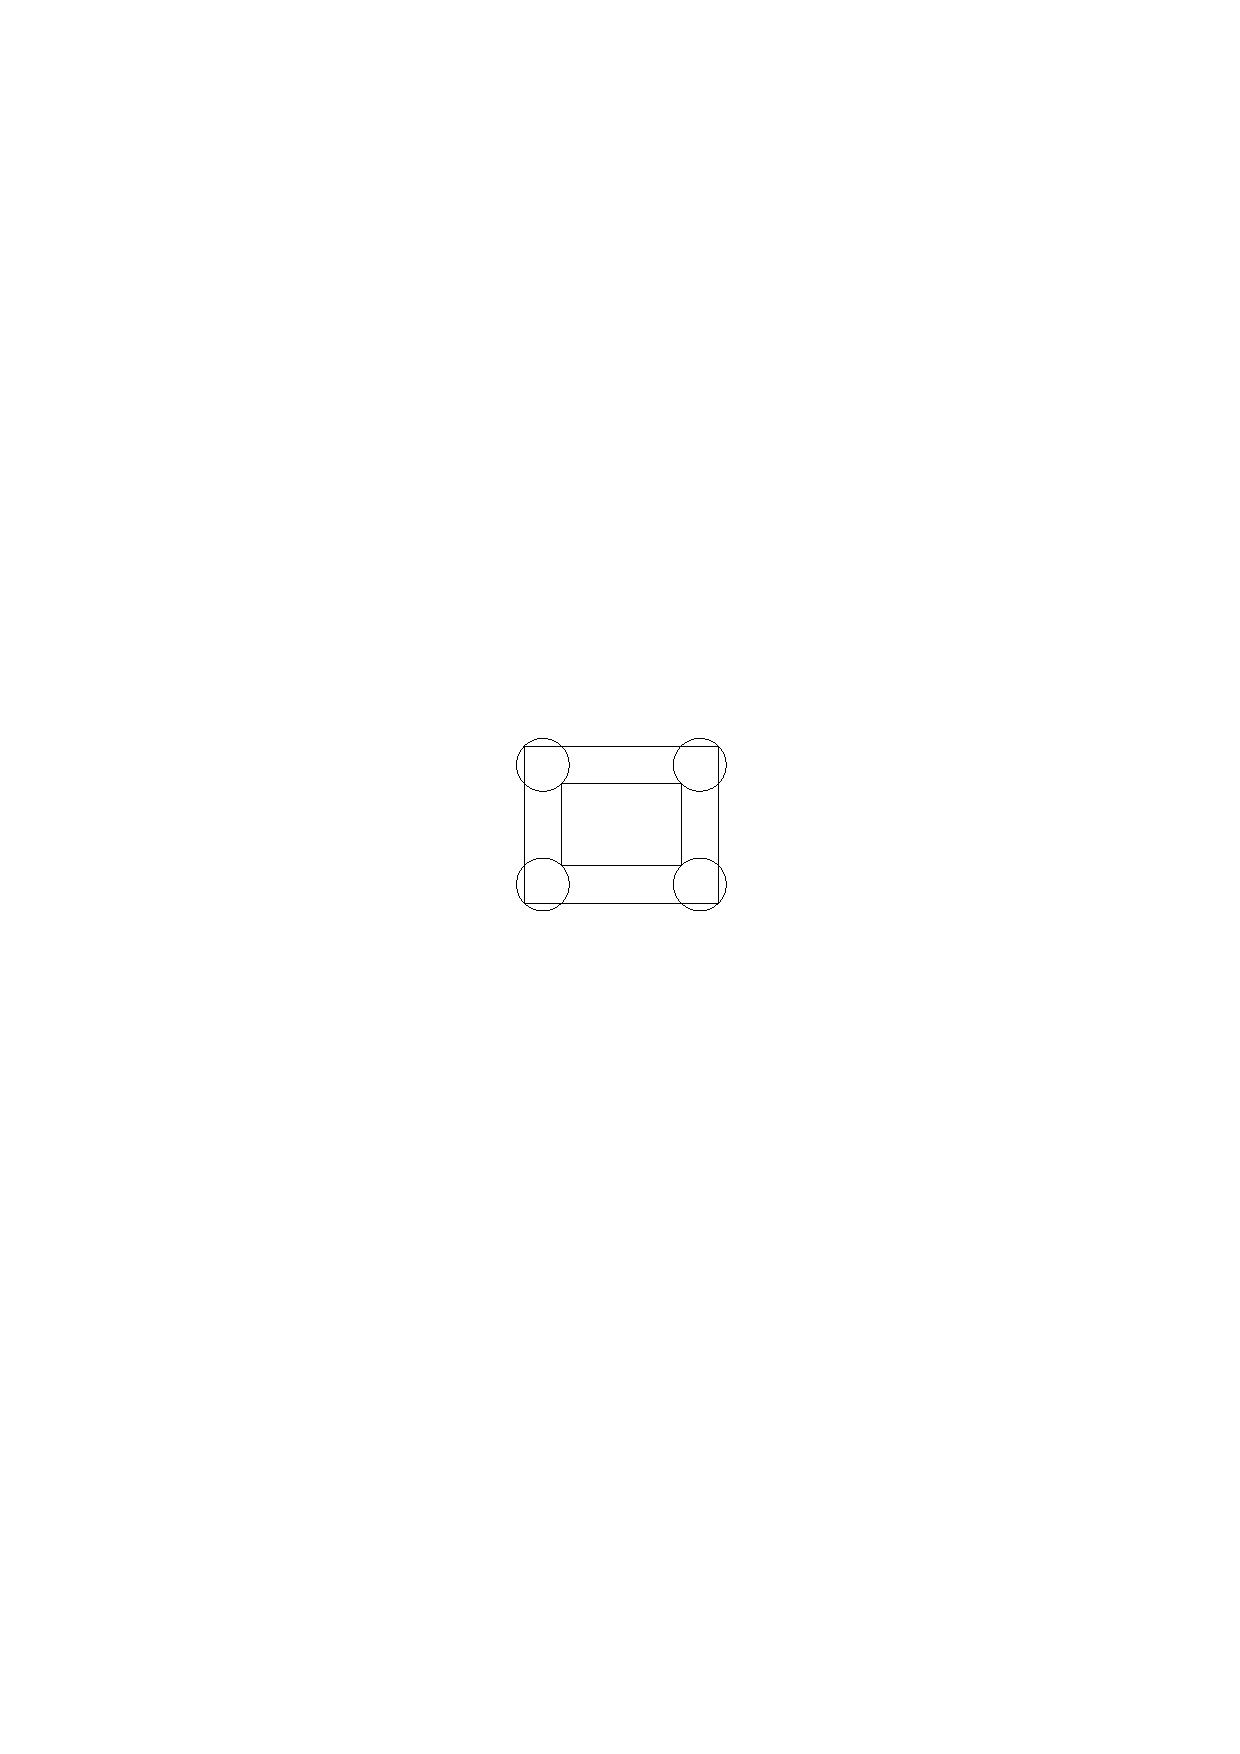
\includegraphics[scale=0.6]{./swirski/castle.pdf}
\end{figure}

\textbf{Nocny strażnik planuje zamkniętą trasę obchodu wzdłuż krawędzi tego grafu.\\
(a) Ile istnieje takich tras (bez uwzględniania kierunku), które przechodzą przez każdy węzeł dokładnie raz?\\
(b) Ile istnieje takich tras (z uwzględnieniem kierunku), które przechodzą przez każdą krawędź dokładnie raz i nie krzyżują się same ze sobą?}
\zrodlo{XXIII Austriacko-Polskie Zawody Matematyczne}

(a) Rozważmy przebieg trasy strażnika w jednym z czterech naroży zamku. Wyróżnimy następujące sytuacje:\\
\\
A: strażnik podczas swojej trasy przechodzi przez naroże dwukrotnie. Przebieg trasy w narożu można ustalić na 4 sposoby.

\begin{figure}[!h]
  \begin{flushright}
  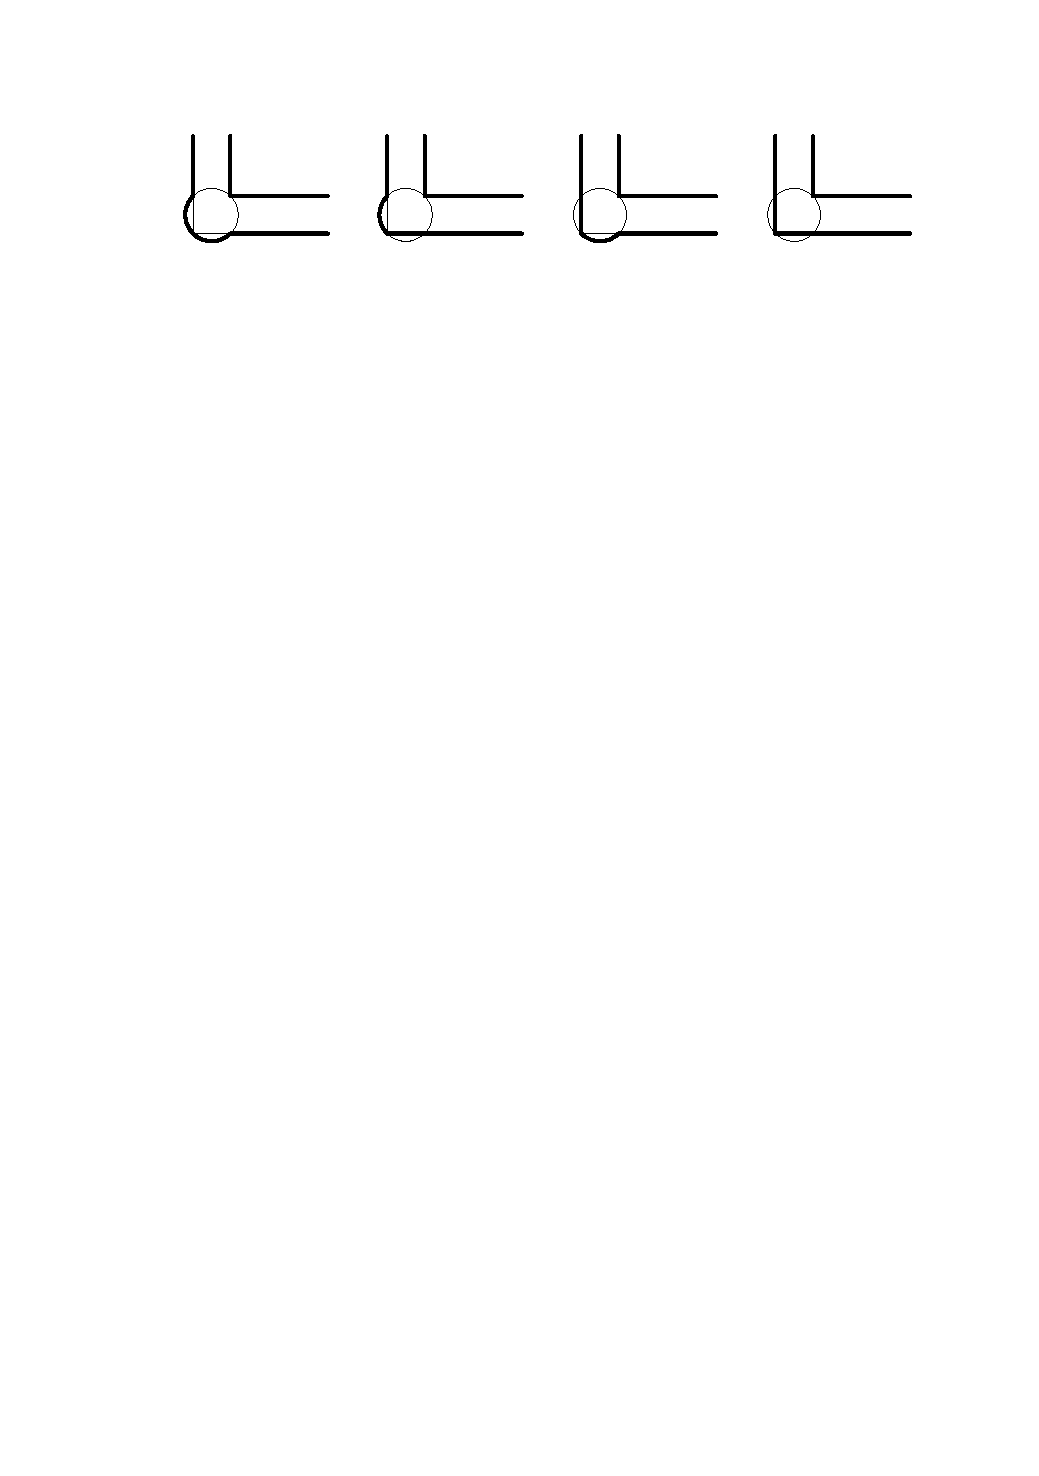
\includegraphics[scale=1]{./swirski/ex6a.pdf}
  \end{flushright}
\end{figure}

B: strażnik przechodzi przez naroże jednokrotnie, przy czym wychodzi
z naroża wracajac w tym samym kierunku, z którego wszedł. Także w tym
wypadku przebieg trasy w narożu można ustalić na 4 sposoby,
o ile ustalony jest kierunek, z którego wchodzi straznik.
\begin{figure}[!h]
  \begin{flushright}
  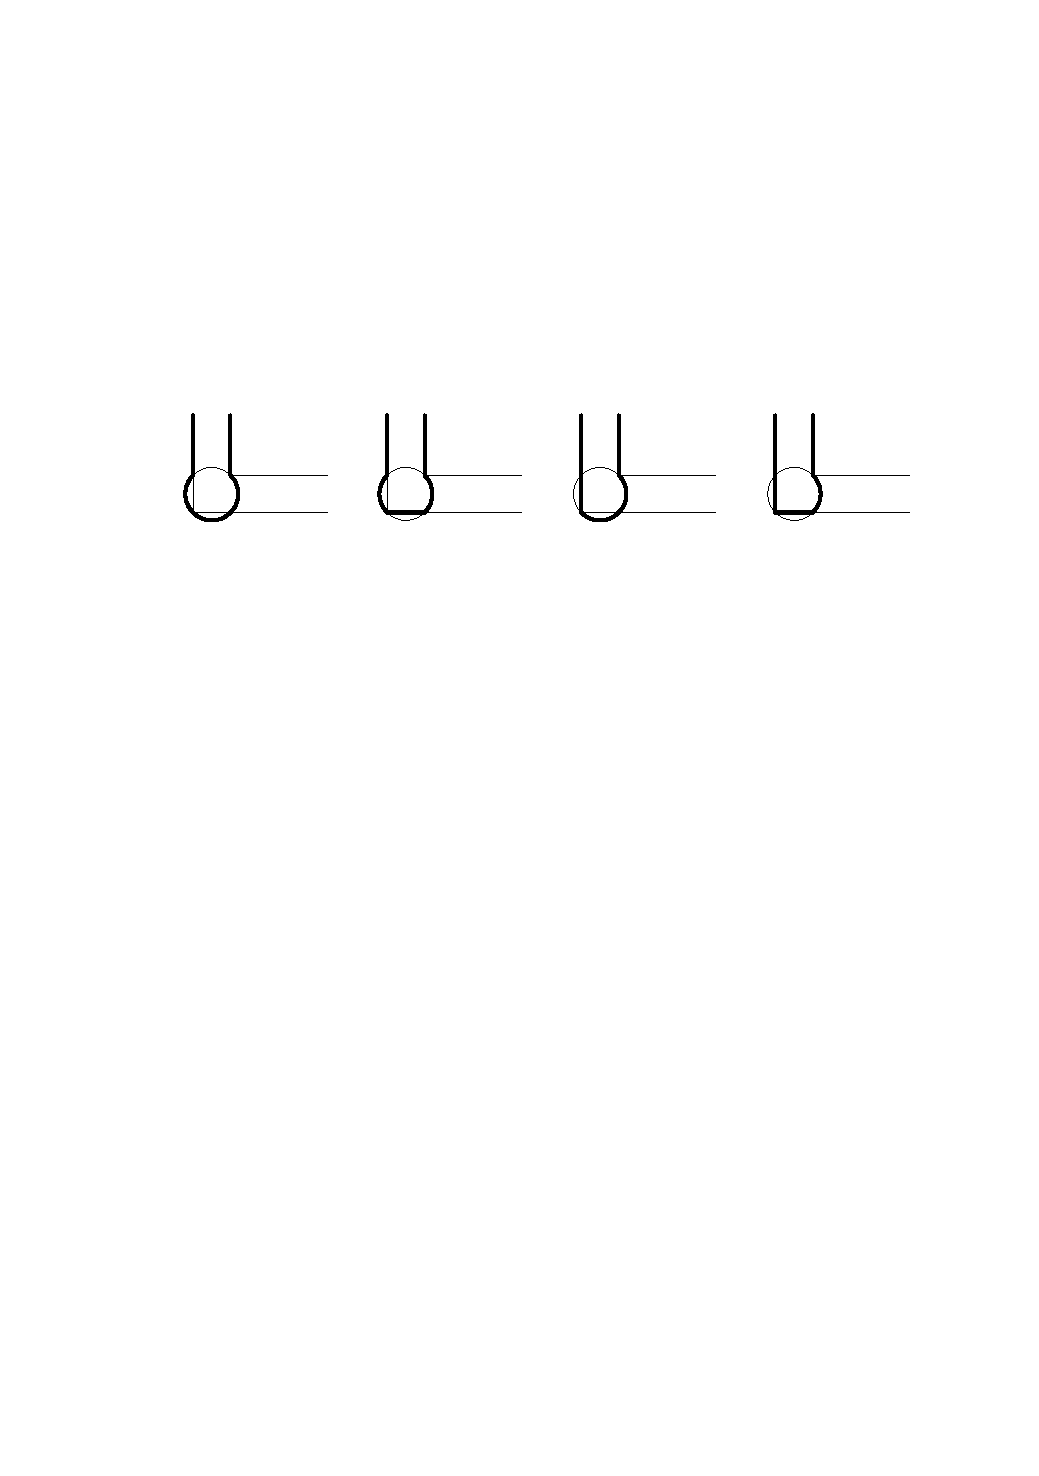
\includegraphics[scale=1]{./swirski/ex6b.pdf}
  \end{flushright}
\end{figure}

C: strażnik przechodzi przez naroże jednokrotnie, przy czym wychodzi
z naroża idąc w przeciwnym kierunku, niż ten, z którego wszedł. Mamy tu
8 możliwych przebiegów trasy, które podzielimy na dwa typy: C1 (górny rząd)
i C2 (dolny rząd).
\begin{figure}[!h]
  \begin{flushright}
  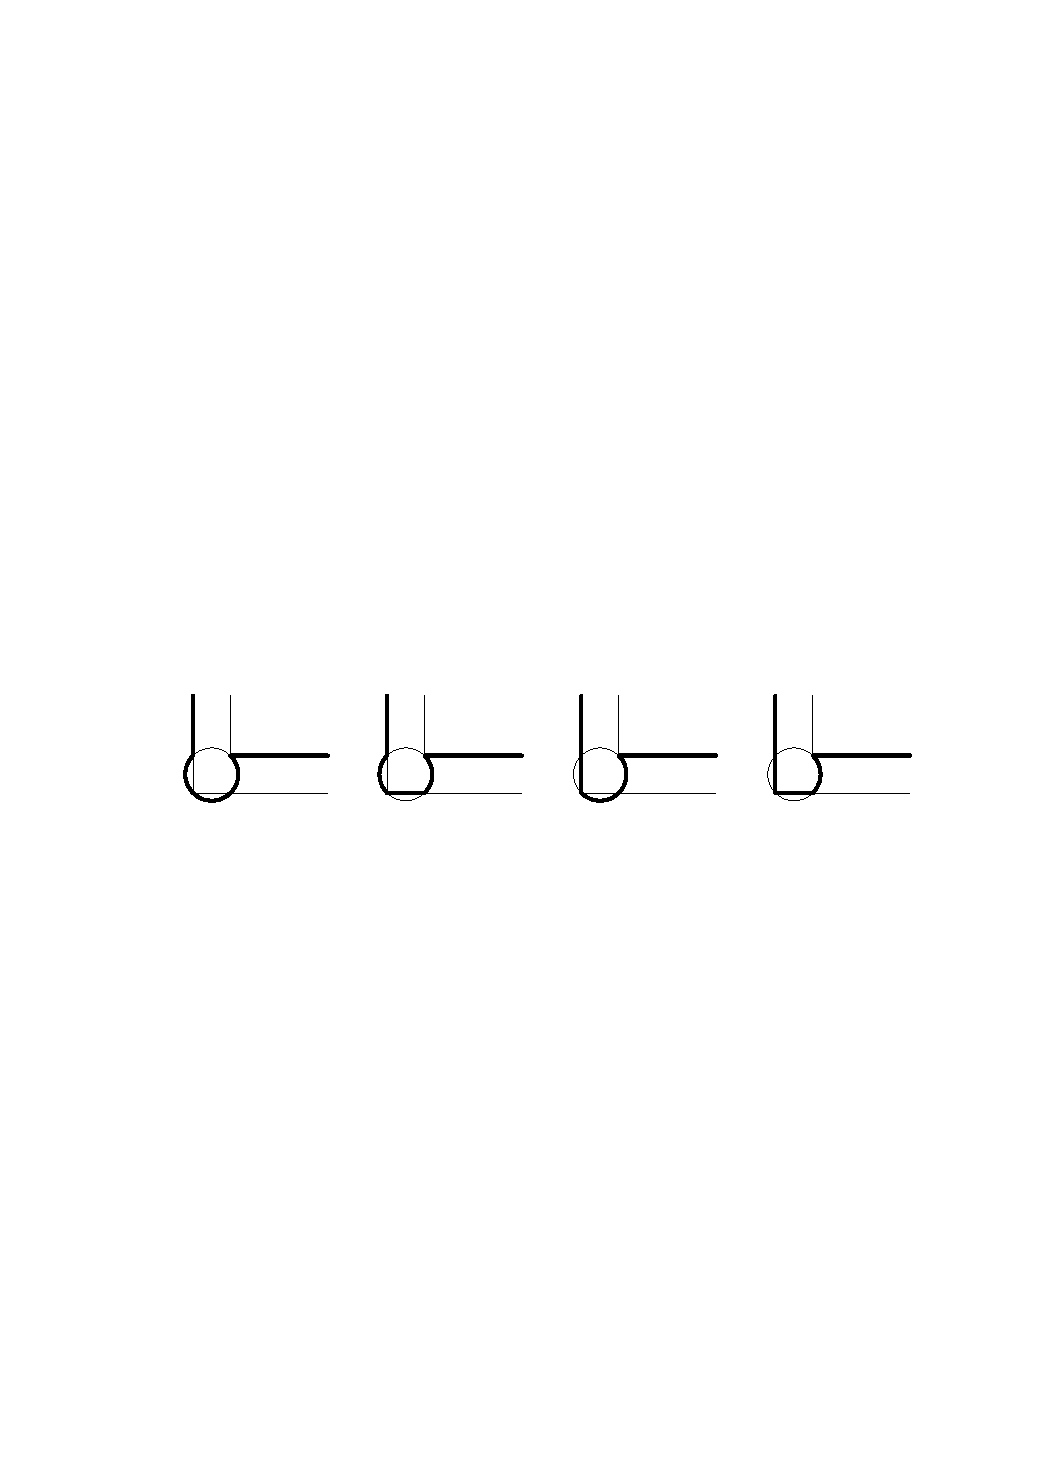
\includegraphics[scale=1]{./swirski/ex6c.pdf}
  \end{flushright}
\end{figure}
\begin{figure}[!h]
  \begin{flushright}
  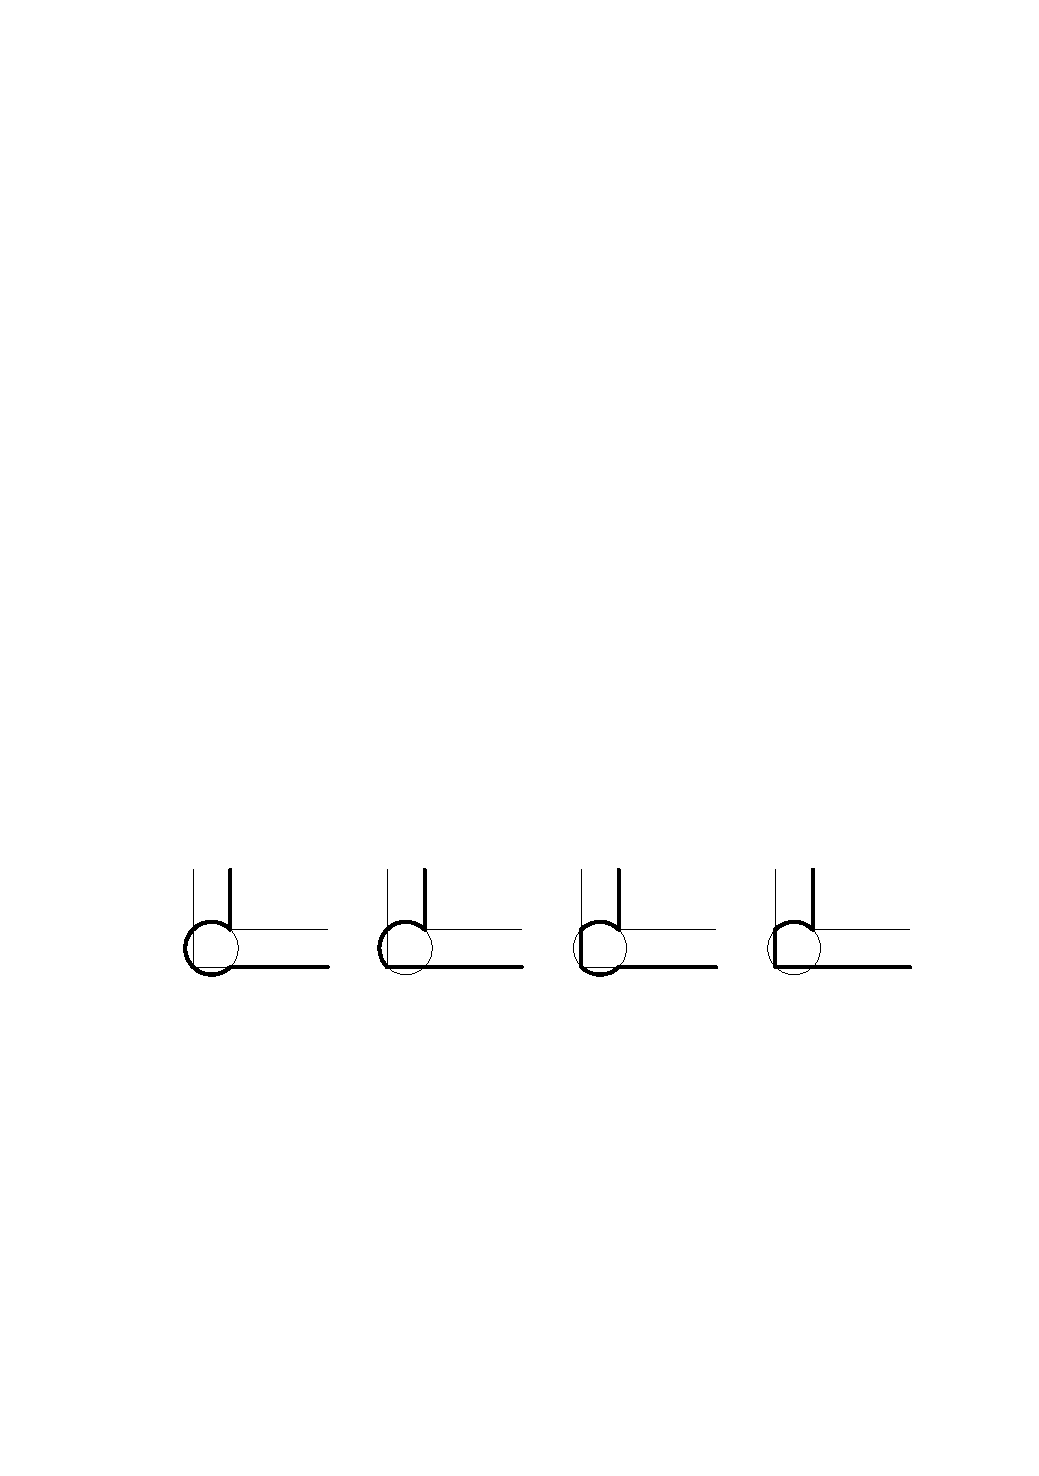
\includegraphics[scale=1]{./swirski/ex6d.pdf}
  \end{flushright}
\end{figure}

Cała trasa strażnika może być cyklem o przejściach przez kolejne naroża typu BAAB, przy czym przypisanie liter A i B narożom może się odbyć na 4 sposoby, a w każdym narożu mamy 4 możliwości zaplanowania trasy. Tak więc otrzymujemy $4 \cdot 4^4 = 1024$ trasy tego typu.

Trasa może też mieć przejścia przez kolejne naroża postaci $C_1C_2C_1C_2$. Przypisanie liter $C_1$ i $C_2$ narożom może się odbywać na dwa sposoby, a w każdym narożu mamy cztery możliwości zaplanowania trasy. Tak więc otrzymujemy $2 \cdot 4^4 = 512$ tras tego typu.

Łącznie liczba tras, które może zaplanować strażnik zgodnie z warunkami
podanymi w części (a), jest równa 1536.

(b) Podobnie jak w pierwszej części zadania, rozważymy przebieg trasy
strażnika w jednym narożu zamku. Wyróżnimy nastepujace sytuacje:

A: wchodząc do naroża korytarzem zewnętrznym opuszczamy naroże korytarzem
zewnętrznym, natomiast wchodząc (po raz drugi) do naroża korytarzem
wewnętrznym wychodzimy także korytarzem wewnętrznym. Przebieg
trasy w narożu można w tym przypadku ustalić na 4 sposoby.
\begin{figure}[!h]
  \begin{flushright}
  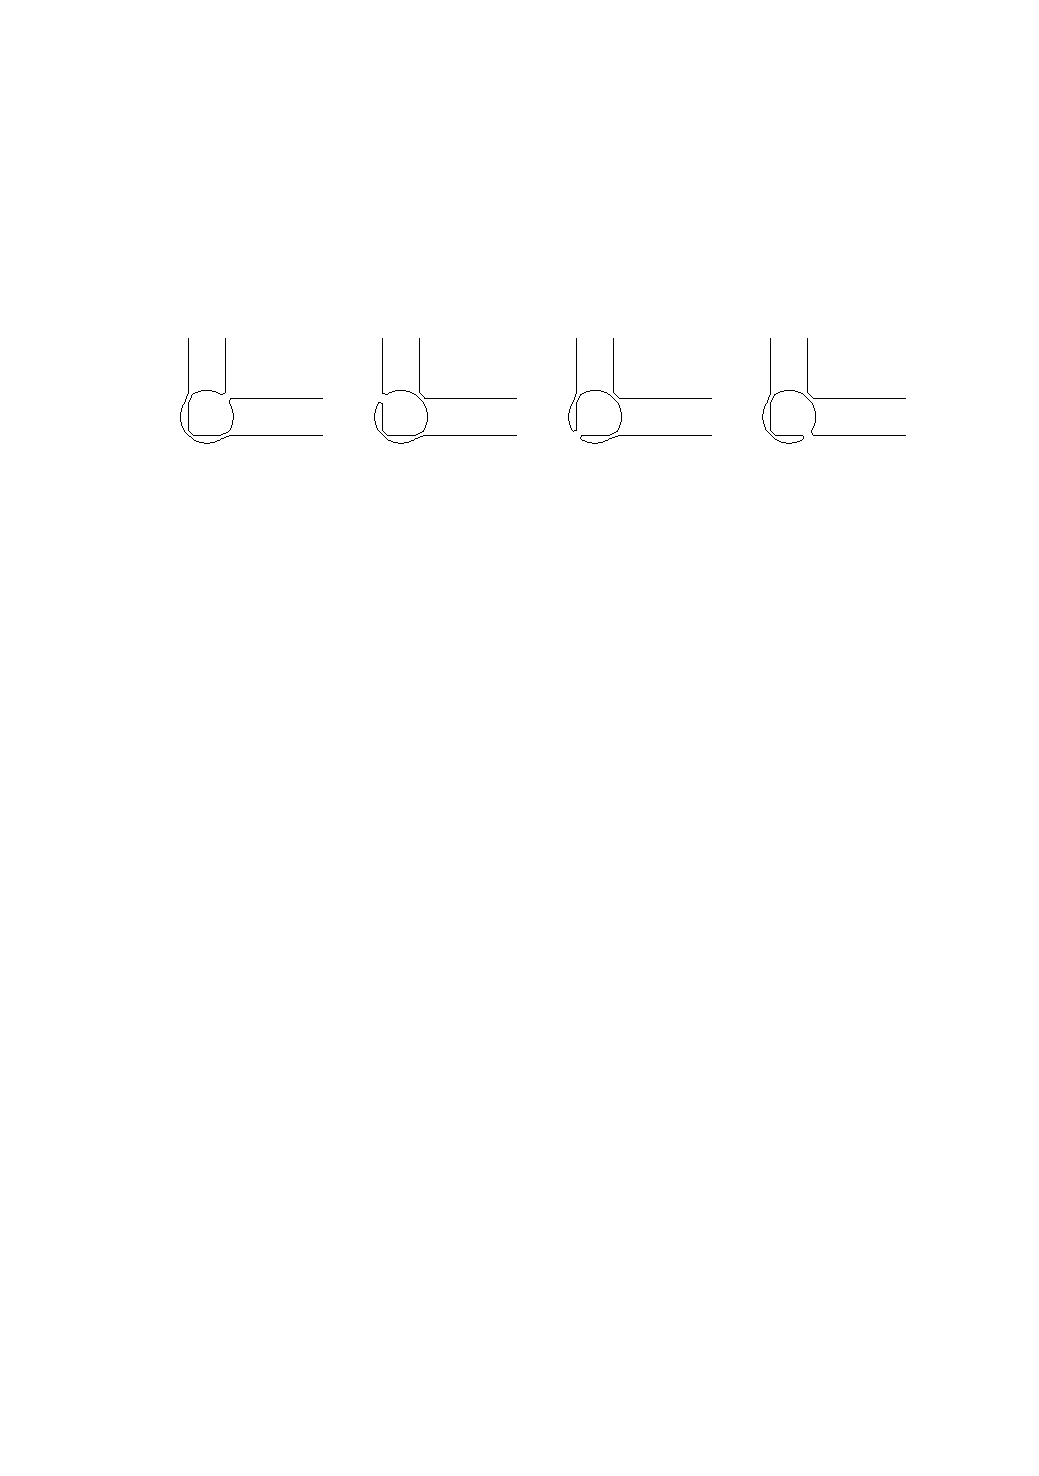
\includegraphics[scale=1]{./swirski/ex6e.pdf}
  \end{flushright}
\end{figure}

B: wchodząc do naroża korytarzem zewnętrznym opuszczamy naroże wracając
korytarzem wewnętrznym (lub na odwrót). Tak samo postepujemy, gdy
po raz drugi znajdziemy sie w narożu. Przebieg trasy w narożu można w tym
przypadku ustalić na 3 sposoby.
\begin{figure}[!h]
  \begin{flushright}
  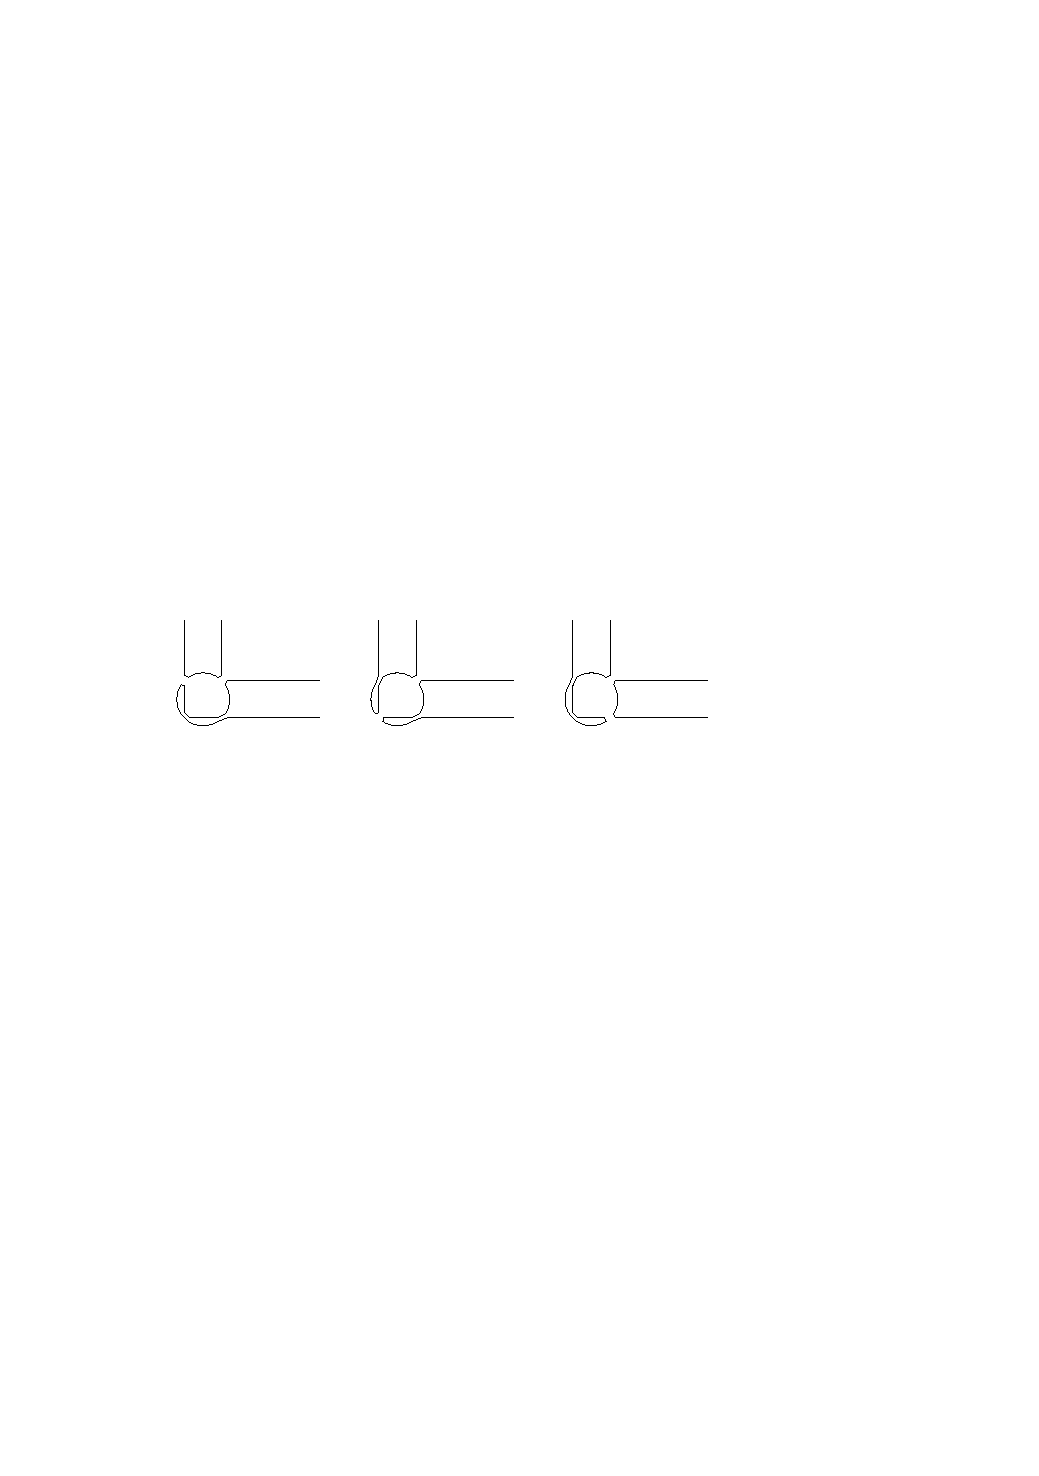
\includegraphics[scale=1]{./swirski/ex6f.pdf}
  \end{flushright}
\end{figure}

Przy planowaniu całej trasy musimy w jednym narożu postąpic według
schematu B, a w pozostałych trzech według schematu A. Zatem łączna liczba
tras (na razie bez uwzględniania kierunku) jest równa $4 \cdot 3 \cdot 4^4 = 768$.

Tak więc liczba tras, które może zaplanować strażnik zgodnie z warunkami
podanymi w częsci (b), jest także równa 1536.

\textit{Uwaga}

Powstaje naturalne pytanie: Czy ta sama odpowiedź w obu częściach zadania
jest dziełem przypadku (któremu zapewne dopomógł autor zadania),
czy też leży za tym jakieś głębsze twierdzenie?

Załóżmy, że zamek ma kształt $n$-kąta foremnego ze strukturą korytarzy
w każdym z $n$ naroży taką samą jak zamek opisany w treści zadania. W części
(a) otrzymamy $n$ schematów typu BAAA \ldots AAAB, co daje $n*4^n$ tras. Schemat
$C_1C_2C_1C_2 \ldots C_1C_2C_1C_2$ występuje dwa razy przy n parzystym, a przy
n nieparzystym nie jest możliwy. Łącznie otrzymujemy w czesci (a) $n\cdot4^n$ lub $(n+2)\cdot4^n$ tras w zależności od parzystości $n$.

Liczba tras w czesci (b) jest równa $2n \cdot 3 \cdot 4^{n-1}$.

Nietrudno sprawdzić, że odpowiedzi w częściach (a) i (b) są równe tylko
dla n=4.

\end{referat}
